
\documentclass[convert={outext=.jpg}]{standalone}
\usepackage{ulem,tikz}
\usetikzlibrary{positioning}

\begin{document}
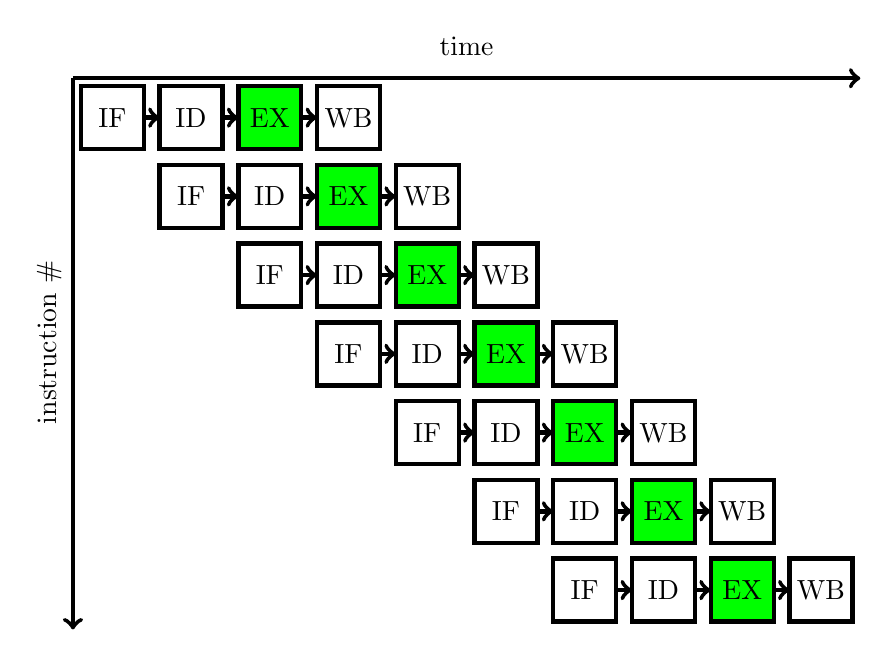
\begin{tikzpicture}[ultra thick]
  \draw [->] (0, 0) -- (10,0) node[midway, label={time}] {};
  \draw [->] (0, 0) -- (0,-7) node[midway,
  label={[rotate=90]instruction \#}] {};
  \foreach \x in {0,...,6}
    {%
      \draw (\x, -\x) ++(0.1,-0.1) rectangle ++(0.8,-0.8)
      node[midway]{IF};
      \draw [->] (\x+0.9,-\x-0.5) -- (\x+1.1,-\x-0.5);
      \draw (\x+1, -\x) ++(0.1,-0.1) rectangle ++(0.8,-0.8)
      node[midway]{ID};
      \draw [->] (\x+1.9,-\x-0.5) -- (\x+2.1,-\x-0.5);
      \draw [fill=green] (\x+2, -\x) ++(0.1,-0.1) rectangle ++(0.8,-0.8)
      node[midway]{EX};
      \draw [->] (\x+2.9,-\x-0.5) -- (\x+3.1,-\x-0.5);
      \draw (\x+3, -\x) ++(0.1,-0.1) rectangle ++(0.8,-0.8)
      node[midway]{WB};
    }%
\end{tikzpicture}
\end{document}
